

\documentclass[9pt]{beamer}
\mode<presentation>
\linespread{1.5}

\usetheme{Madrid}
%\usetheme {CambridgeUS}%{Goettingen}%{Berkeley}%{Montpellier}%{Antibes}%{Dresden}%{Madrid}%{Dresden}%{Darmstadt}%{Warsaw}%{Pittsburgh}
\usefonttheme{{structuresmallcapsserif}}%{structureitalicserif}%{structurebold}%{structuresmallcapsserif}%{professionalfonts}
%\useoutertheme[subsection=false]{smoothbars}
\usepackage[english]{babel}
%\usepackage[latin1]{inputenc}
\usepackage{hyperref}
%\usecolortheme{beaver}
%\usecolortheme{crane}

%\setbeamercovered{transparent}
%\newcommand{\semitransp}[2][35]{\color{fg!#1}#2}

\usepackage{latexsym}
\usepackage{amsmath}
\usepackage{times}
%\usepackage{MinionPro}
\usepackage{hyperref}
\usepackage{tikz}
\usepackage{verbatim}
\usepackage{natbib}
\usepackage{color, colortbl}
\usepackage{appendix}
\usepackage{ulem}
\usepackage{amsmath,amsthm}
\usepackage{bbm}
\usetikzlibrary{arrows,shapes}


\newtheorem{proposition}{Proposition}[section]
%\newtheorem{definition}{Definition}[section]
\newtheorem{assumption}{Assumption}[section]
\newtheorem{conjecture}{Conjecture}[section]
\newtheorem*{observation}{Observation}


\definecolor{Gray}{gray}{0.9}


\pgfdeclarelayer{background}
\pgfsetlayers{background,main}

\tikzstyle{vertex}=[circle,fill=black!25,minimum size=12pt,inner sep=0pt]
\tikzstyle{selected vertex} = [vertex, fill=red!24]
\tikzstyle{unknown vertex} = [vertex, fill=black]
\tikzstyle{edge} = [draw,thick,-]
\tikzstyle{weight} = [font=\small]
\tikzstyle{selected edge} = [draw,line width=5pt,-,red!50]
\tikzstyle{ignored edge} = [draw,line width=5pt,-,black!20]







\title{Coordination in Social Networks}
\author{Chun-Ting Chen}


\begin{document}

\maketitle


\section{Introduction}
\subsection{Motivation}


\frame{
  \frametitle{Motivation}

\begin{itemize}
\item An exogenous social network models \textbf{restricted information} \onslide<2->{\textcolor{blue}{in repeated collective action}}
\begin{table}[h]
\begin{tabular}{ll }
\onslide<1>{~[Chwe] models}  & \textbf{incomplete information} \\
\onslide<1>{~[Wolitzky] models} &  \textbf{network-monitoring}
\end{tabular}
\end{table}

%\begin{itemize}
%\item \onslide<1>{~[Chwe] models} \textbf{incomplete information}.
%\item \onslide<1>{~[Wolitzky] models} \textbf{network-monitoring}.
%\end{itemize}

\pause
\item Will people solve the uncertainty and act collectively in networks \textcolor{blue}{eventually}?
\pause
\item This paper provides \textcolor{blue}{a partial folk theorem} with {incomplete information} and {network-monitoring}.

\end{itemize}

}


\frame{
  \frametitle{What this paper does?}
\alert{Model}: repeated game of private provision of public good
\begin{itemize}
\item Players are allocated in a fixed and exogenous network.
\pause
\item Time line
\begin{itemize}
\item Nature choose a type distribution
\item Types are then fixed over time
\item Players play a ``public good provision game'' infinitely repeatedly with common discount factor.
\end{itemize}





\end{itemize}

}

\frame{
  \frametitle{What this paper does?}
\alert{Stage game}: Features
\begin{itemize}[<+->]


\item Players of two types: \textbf{Strategic type}/\textbf{Behavior type}
\begin{table}[h]
\begin{tabular}{ll}
Strategic type & \textbf{provide}/\textbf{not to provide}  \\
Behavior type &  \textbf{not to provide} 
\end{tabular}
\end{table}
\item Strategic type's stage pay-off $u$:
\[u(\textit{own action},\mathbbm{1}(\textit{sufficient provision of public good}))\]


\end{itemize}

}

\frame{
  \frametitle{What this paper does?}
\alert{Network-information-structure}: 

\begin{table}[h]
\begin{tabular}{l}
\textbf{own/neighbors' types} is perfectly observable \\
\textbf{own/neighbors' actions} is perfectly observable
\end{tabular}
\end{table}



\alert{Goal}: looking for an equilibrium, in which the global type distribution becomes commonly known in finite time.
\\
\bigskip
\alert{Result}: such equilibrium can be constructed under some assumptions.



}




\section{Model}
\subsection{Model}



\frame{
  \frametitle{Model}
\begin{itemize}
\item A fixed and finite network
  \begin{itemize}
\item $n$ players; $N=\{1,...,n\}$ is the set of players. 
  \item $G_i$ is $i$'s neighborhood; $G_i$ is a subset of $N$ such that $i\in G_i$.
  
  \item $G=\{G_i\}_i$ is the network.
 
  \end{itemize}

\item Players of two types
\begin{itemize}
\item Player $i$'s type: $\theta_i\in \Theta_i=\{S,B\}$.
\item Type-contingent action set:  $A_{S}=\{\textbf{p},\textbf{np}\}$; $A_{B}=\{\textbf{np}\}$
\item Type profile: $\theta\in \Theta=\times_{i\in N}\Theta_i$
\end{itemize}
\end{itemize}

}




\begin{frame}[label=static_game]
  \frametitle{Model}
Stage game: $k$-threshold game

  \begin{itemize}

  \item Stage game payoff for S-type $i$: $u_{S_i}(a_{S_i},a_{-\theta_i})$

\end{itemize}
  \begin{table}[h]
\begin{tabular}{llll}
$u_{S_i}(a_{S_i},a_{-\theta_i})$ & $=$ & 1 & if $a_{S_i}=\textbf{p}$ and $\#\{j:a_{\theta_j}=\textbf{p}\}\geq k$ \\
$u_{S_i}(a_{S_i},a_{-\theta_i})$ & $=$ & -1 & if $a_{S_i}=\textbf{p}$ and $\#\{j:a_{\theta_j}=\textbf{p}\}< k$ \\
\\
$u_{S_i}(a_{S_i},a_{-\theta_i})$ & $=$ & 0 & if $a_{S_i}=\textbf{np}$ \pause \\
\end{tabular}

\end{table}


 \begin{itemize}
 \item Ex-post efficient outcome: 
 \begin{table}[h]
\begin{tabular}{ll}
relevant information & ex-post efficient outcome \\
\hline
At least $k$ S-types exist & All S-types play \textbf{p}  \\
Otherwise &  All S-types play \textbf{np} 
\end{tabular}
\end{table}

 \end{itemize}

\end{frame}







\subsection{Repeated Game}


\begin{frame}
  \frametitle{Model}

Assumptions:
\begin{itemize}
\item Network $G$ is \alert{commonly known}, \alert{connected}, and \alert{undirected}.
\item A common prior: $\pi\in \Delta \Theta$
\item A common discount factor: $\delta\in (0,1)$.
\item Players perfectly observe their neighbors' types.
\item Players perfectly observe their neighbors' actions. 
\end{itemize}


\end{frame}


\begin{frame}
  \frametitle{Goal}

Look for
\begin{itemize}
\item \textbf{An equilibrium, the ex-post efficient outcome repeats after some \alert{finite time $T$} in the path} (\textcolor{blue}{APEX}). \pause
\[\Downarrow\onslide<3>{{\Uparrow}(\text{with some additional assumptions})}\]
\item \textbf{The relevant information must be \alert{commonly known after $T$} in the path}.  
\end{itemize}

\end{frame}







\begin{frame}
  \frametitle{Notations}

Notations:
\begin{itemize}

\item $\alert{\theta_{G_i}}\in \Theta_{G_i}$: $i$'s private information about the state. 
\item $\alert{h^{m}_{G_i}}\in H^m_{G_i}$: the history of actions observed by $i$ up to period $m$.
\item \alert{$\Theta_{G_i}\times H^m_{G_i}$}: $i$'s observation up to time $m$.
\pause
\item $h^m$: a sequence of players' actions up to period $m$.
\item $h$: an infinite sequence of players' actions. 




 
\end{itemize}

\end{frame}




\begin{frame}
  \frametitle{APEX strategy path}
Notations:
\begin{itemize}
\item $\tau_i:\Theta_{G_i}\times \bigcup^{\infty}_{m=0} H^{m}_{G_i} \rightarrow A_{\theta_i}$, $i$'s strategy.
\item $\tau=(\tau_1,...,\tau_i,...,\tau_n)$: a strategy profile. 
\item $h^{\tau}_{\theta}$ : a history generated by $\tau$ given $\theta$.
\item $\tau$-path: $\{h^{\tau}_{\theta}\}_{\theta\in \Theta}$
\end{itemize}

\begin{definition}
The $\tau$-path is \textbf{approaching ex-post efficient} (\textcolor{blue}{\textit{APEX}}) $\Leftrightarrow$ 
\[\text{$\forall\theta$,  there is a finite time $T^{\theta}$}\] 
such that the actions after $T^{\theta}$ in $h^{\tau}_{\theta}$ repeats the static ex-post efficient outcome.
\end{definition}


\end{frame}




\begin{frame}
  \frametitle{Equilibrium Concept}

Notations:
\begin{itemize}

\item $\beta^{\pi,\tau}_i(\theta|h^{m}_{G_i})$: $i$'s belief for a $\theta$ at period $m$ given $\pi,\tau$.
\item $\phi_{G_i}: H^m\rightarrow H^m_{G_i}$: the projection mapping a $h^m$ to $h^m_{G_i}$.
\end{itemize}

\begin{definition}
$h^m_{G_i}$ is \textbf{reached} by $\tau$ iff there is a pair $(\theta,h^m)$ such that $h^m$ is on the $\tau$-path, and $h^m_{G_i}=\phi_{G_i}(h^m)$. 
\end{definition}


\end{frame}


\begin{frame}
  \frametitle{Equilibrium Concept}


\begin{definition}[weak sequential equilibrium]
The pair $(\tau^{*},\beta^{*})$, 
\begin{itemize}
\item $\tau^{*}$: a strategy
\item $\beta^{*}=\{\beta^{*,m}\}_m$: the belief system 
\begin{itemize}
\item $\beta^{*,m}_i$: $\Theta_{G_i}\times H^{m}_{G_i} \rightarrow \Delta (\Theta\times H^m)$
\end{itemize}
\end{itemize}

, is a weak sequential equilibrium iff
\begin{itemize}
\item $\beta^{*,m}_i(\theta|h^{m}_{G_i})=\beta^{\pi,\tau^{*}}_i(\theta|h^{m}_{G_i})$ whenever $h^{m}_{G_i}$ is reached by $\tau^{*}$ for all $i$.
\item $\tau^{*}$ is sequential rational given $\beta^{*}$.
\end{itemize}





\end{definition}




\end{frame}


\begin{frame}
  \frametitle{Equilibrium Concept}


\begin{definition}[Sequential equilibrium]
A sequential equilibrium $(\tau^{*},\beta^{*})$  is a weak  sequential equilibrium and $\beta^{*}$ is fully consistent with $\tau^{*}$[Krep and Wilson].
\end{definition}
\begin{itemize}
\item Fully consistent: 
the $\beta^{*}$ is \textbf{``very very similar with''} that belief system induced by a \textbf{``very very little perturbed''} strategies around $\tau^{*}$.
\end{itemize}
\end{frame}

\begin{frame}
  \frametitle{APEX Equilibrium}

\begin{itemize}
\item Finally, let the ``(weak) APEX equilibrium'' be \textcolor{blue}{the (weak) sequential equilibrium in which the equilibrium path is APEX}.
\item Does an APEX equilibrium exist?
\end{itemize}

\end{frame}

\begin{frame}


  \frametitle{Outline}
Outline

\begin{itemize}
\item An example for APEX equilibrium
\item Result 1: APEX equilibrium for $k=n$.
\item Result 2: weak APEX equilibrium for $k<n$.
\begin{itemize}
\item Idea in equilibrium construction: introducing a ``mailing game''
\item Sketch of proof.
\end{itemize}
\item Extension
\item Further works
\end{itemize}


\end{frame}



\begin{frame}
  \frametitle{Leading example}
\begin{itemize}
\item Let $G=$
\begin{center}
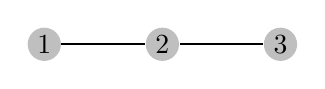
\begin{tikzpicture}[scale=1.5]
    % Draw a 7,11 network
    % First we draw the vertices
    \foreach \pos/\name in {{(1,0)/1}, {(2,0)/2}, {(3,0)/3}}
        \node[vertex] (\name) at \pos {$\name$};
    % Connect vertices with edges 
    \foreach \source/ \dest in {1/2, 2/3}
        \path[edge] (\source) -- (\dest) ;
        
\end{tikzpicture}
\end{center}
\item Let $k=n=3$.
\end{itemize}
  
An APEX equilibrium can be constructed by
\begin{itemize}



\item At period 1
\begin{itemize}
\item S-type 2: $\textbf{p}$ in $\theta=(S,S,S)$;
\item S-type 2: $\textbf{np}$ in $\theta\neq (S,S,S)$, and then \alert<2>{\textbf{np} forever\onslide<2>{\textcolor{blue}{ (the state is revealed)}}}
\item S-type 1 (or S-type 3): \textbf{np}.
\end{itemize}

\item After period 1
\begin{itemize}
\item If S-type 2 chooses \textbf{p} in the last period, then S-type 1 (or S-type 3) chooses \textbf{p} forever; 
\item If S-type 2 chooses \textbf{np} in the last period, then S-type 1 (or S-type 3) chooses \alert<2>{\textbf{np} forever \onslide<2>{\textcolor{blue}{ (undetectable deviation)}}}.
\end{itemize}
 
 \item Any deviation $\Rightarrow$ Choosing \alert<2>{\textbf{np} forever\onslide<2>{\textcolor{blue}{ (detectable deviation)}}}.
\end{itemize}

\end{frame}


\begin{frame}
  \frametitle{Leading example}
Main features in equilibrium construction
\begin{itemize}
\item Actions (in first period) serve as ``\textcolor{blue}{messages}'' to reveal the relevant information.
\item The ``\textcolor{blue}{timing}'' (second period) to coordinate to ex-post efficient outcome is part of equilibrium strategy.  
\item Playing \textbf{np} forever serves as a ``\textcolor{blue}{grim trigger}''.
\end{itemize}  
\end{frame}


\frame{
  \frametitle{Result 1: APEX for $k=n$}

\begin{theorem}[\alert{$k=n$}]

In any network, if  the prior has full support, then for repeated $k=n$ Threshold game, an APEX equilibrium exists whenever $\delta$ is sufficiently high.
\end{theorem}

Sketch of proof:
  \begin{enumerate}
  
\item ``messages'' to reveal the relevant information.
\begin{itemize}
  \item Some B-types neighbors $\Rightarrow$ play \textbf{np} forever.
  \item No B-type neighbor $\Rightarrow$ play \textbf{p} until \textbf{np} is observed, and then play \textbf{np} forever.
\end{itemize}
\pause
\item The ``timing'' to coordinate.
\begin{itemize}
 \item Finite network $\Rightarrow$ there is a finite time $T^{\theta}$ such that players coordinate to ex-post efficient outcome.
\end{itemize}
 \pause
  \item Any deviation $\Rightarrow$ play \textbf{np} forever.
  \pause
  \item A fully consistent belief system can be chosen.
   \end{enumerate}

}




\frame{
  \frametitle{Result 2: APEX for $k<n$}

\begin{theorem}[\alert{$k< n$}]
\label{thm_main_result}
In any \alert{acyclic} network, if $\pi$ has \alert{full support on strong connectedness}, then for repeated $k<n$ Threshold game, a {weak} APEX equilibrium {exists} whenever $\delta$ is sufficiently high.
\end{theorem}
Main difficulties
\begin{itemize}
\item Using sequence of \textcolor{blue}{binary actions to reveal how many S-types out there}.
\item These sequences has to be \textcolor{blue}{incentive compatible}.
\item \textcolor{blue}{Explicitly calculating the timing to coordination} may be intractable.
\item Due to \textcolor{blue}{network-monitoring}, group punishment is hard to be made.
\end{itemize}
Main idea
\begin{itemize}
\item Consider a simple version of equilibrium construction in a ``\alert{mailing game}''.
\end{itemize}
}


\begin{frame}
  \frametitle{Acyclic network}


\begin{definition}[Path in a network]
A \textbf{path} from node $i$ to node $j$ is a sequence of nodes \[\{i,m_1,m_2,...,m_n,j\} \text{ without repetition }\] such that $i\in G_{m_1},m_1\in G_{m_2},...,m_n\in G_j$. 
\end{definition}  

\begin{definition}[Acyclic network (Tree)]
A network is \textbf{acyclic} $\Leftrightarrow$ the path from node $i$ to node $j$ is unique for all nodes $i,j$. 
\end{definition}  

\end{frame}





\begin{frame}
  \frametitle{Strong connectedness}


\begin{definition}
$\theta$ has \textbf{strong connectedness}$\Leftrightarrow$ for every pair of S-types, there is a path consisting of S-types to connect them.
\end{definition}  

\begin{definition}
$\pi$ has \textbf{full support on strong connectedness}$\Leftrightarrow$ 
\[\text{$\pi(\theta)>0$ \textbf{if and only if} $\theta$ has strong connectedness.}\]
\end{definition}  
\pause

\begin{itemize}
\item An B-type will not reveal information.
\item Without \textbf{full support on strong connectedness}, in general, an Apex equilibrium does not exist when pay-off (as a signal) is hidden or noisy.
\item Ex. $k=2$. $G$ and $\theta=$
\begin{center}
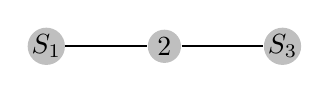
\begin{tikzpicture}[scale=1.5]
    % Draw a 7,11 network
    % First we draw the vertices
    \foreach \pos/\name in {{(1,0)/S_1}, {(2,0)/2}, {(3,0)/S_3}}
        \node[vertex] (\name) at \pos {$\name$};
    % Connect vertices with edges 
    \foreach \source/ \dest in {S_1/2, 2/S_3}
        \path[edge] (\source) -- (\dest) ;
        
\end{tikzpicture}
\end{center}
\end{itemize}
\end{frame}




\section{Equilibrium construction}
\subsection{Equilibrium construction}


\begin{frame}
  \frametitle{$T$-period Mailing game}

\begin{itemize}
\item A fixed and commonly known number $T$, where $T$ is big enough.


\item A fixed and finite network
  \begin{itemize}
\item $n$ players; $N=\{1,...,n\}$ is the set of players. 
  \item $G_i$ is $i$'s neighborhood; $G_i$ is a subset of $N$ such that $i\in G_i$.
  
  \item $G=\{G_i\}_i$ is the network.
 
  \end{itemize}

\item Players of two types
\begin{itemize}
\item Player $i$'s type: $\theta_i\in \Theta_i=\{S,B\}$.
\item Type profile: $\theta\in \Theta=\times_{i\in N}\Theta_i$.
\item A common prior over $\Theta$: $\pi$
\end{itemize}



\end{itemize}

\end{frame}



\begin{frame}
  \frametitle{$T$-period Mailing game}

\begin{itemize}

\item A ``letter-writing technology'' for player $i$:
\begin{itemize}
\item A set of sentences: $W=\{n,p\}^L$, where $L$ is a big number.
\item $M^1_i=\{f|f:\Theta_{G_i}\rightarrow W\}$; $M^{t+1}_i=\{f|f\text{ is a selection from }\prod_{j\in G_i}M^{t}_j\}$ for $T\geq t\geq 1$.
\end{itemize}

\item Type-contingent action set for player $i$:
\begin{itemize}
\item $A^t_{S_i}=\{\textbf{send},\textbf{hold}\}\times M^t_i$; $A^t_{B_i}=\{\textbf{hold}\}$, for $t\geq 0$.
\end{itemize}

\item A ``letter-sending technology'' for player $i$:
\begin{itemize}
\item If $(\textbf{send},m^t_i)$ is chosen, a fixed cost of $\epsilon$ incurs, where $\epsilon$ is small enough.
\item If $(\textbf{send},m^t_i)$ is chosen, $m^t_i$ is observable by $G_i$.
\item If $(\textbf{hold},m^t_i)$ is chosen, no cost incurs and $m^t_i$ is not observable by $G_i$.
\end{itemize}
\end{itemize}

\end{frame}


\begin{frame}
  \frametitle{$k$-Threshold game augmented by $T$-period Mailing game}

Time line
\begin{itemize}

\item Nature choose $\theta$ according to $\pi$.
\item Types are then fixed over time.
\item At the first $T$ periods, players play $T$-period Mailing game.
\item At $T+1$ period, players play a one-shot $k$-Threshold game.
\item Game ends.
\end{itemize}

\end{frame}


\begin{frame}
  \frametitle{$k$-Threshold game augmented by $T$-period Mailing game}
Example of a weak equilibrium construction:
\begin{itemize}
\item Let $k=5$, $T=2$.
\item Suppose $G$ and $\theta$=
\begin{center}
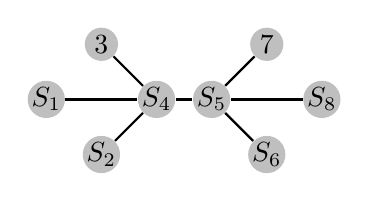
\begin{tikzpicture}[scale=0.7]
    % Draw a 7,11 network
    % First we draw the vertices
    \foreach \pos/\name in {{(1,2)/S_1}, {(2,1)/S_2}, {(2,3)/3}, {(5,1)/S_6}, {(5,3)/7}, {(6,2)/S_8}, {(3,2)/S_4}, {(4,2)/S_5}}
        \node[vertex] (\name) at \pos {$\name$};
    
%    \foreach \pos/\name in {{(3,2)/S_4}, {(4,2)/S_5}}
%    \node[selected vertex] (\name) at \pos {$\name$};
    
    % Connect vertices with edges 
    \foreach \source/ \dest in {S_1/S_4, S_2/S_4,3/S_4,S_4/S_5, S_5/S_6, S_5/7, S_5/S_8}
        \path[edge] (\source) -- (\dest) ;
        
\end{tikzpicture}
\end{center}
\end{itemize}

\begin{itemize}
\item Equilibrium path
\begin{itemize}
\item \alt<2>
{At \textcolor{blue}{$t=2$}, 
\begin{table}[h]
\begin{tabular}{ll l}
S-type 4 & (\textbf{send} & $(\overbrace{n,n,...,\underbrace{p,n,...,n}_{\textcolor{blue}{4}}}^{L})$, $(\overbrace{n,n,...,\underbrace{p,n,...,n}_{\textcolor{blue}{4}}}^{L})$ )\\
S-type 5 & (\textbf{send} & $(\overbrace{n,n,...,\underbrace{p,n,...,n}_{\textcolor{blue}{4}}}^{L})$, $(\overbrace{n,n,...,\underbrace{p,n,...,n}_{\textcolor{blue}{4}}}^{L})$ )\\
S-type 1,2,6,8 & (\textbf{not send} & $(\overbrace{n,n,...,n,n,...,n}^{L})$, $(\overbrace{n,n,...,n,n,...,n}^{L})$ )
\end{tabular}
\end{table}
}
{At \textcolor{blue}{$t=1$}, 
\begin{table}[h]
\begin{tabular}{ll l}
S-type 4 & (\textbf{send} & $(\overbrace{n,n,...,\underbrace{p,n,...,n}_{\textcolor{blue}{4}}}^{L})$ )\\
S-type 5 & (\textbf{send} & $(\overbrace{n,n,...,\underbrace{p,n,...,n}_{\textcolor{blue}{4}}}^{L})$ )\\
S-type 1,2,6,8 & (\textbf{not send} & $(\overbrace{n,n,...,n,n,...,n}^{L})$ )
\end{tabular}
\end{table}}


\end{itemize}

\end{itemize}



\end{frame}


\begin{frame}
  \frametitle{$k$-Threshold game augmented by $T$-period Mailing game}


\begin{itemize}
\item Equilibrium path (conti.)
\begin{itemize}
\item At \textcolor{blue}{$t=3$}, all S-types play \textbf{p}
\end{itemize}
\item Off-path strategy
\begin{itemize}
\item If S-type 4 (or 5) make detectable deviation $\Rightarrow$ others play \textbf{hold} and then \textbf{np}.
\item If S-type 4 (or 5) make undetectable deviation $\Rightarrow$ he is facing a possibility of failure to coordinate to \textbf{p}.
\end{itemize}
\item Off-path belief
\begin{itemize}
\item Detectable deviation $\Rightarrow$ believing that all players outside neighborhood are B-types. 
\end{itemize}
\end{itemize}
\pause
\alert{So}, when \textcolor{red}{$\epsilon$ is small enough and $T$ is large enough}, an weak equilibrium can be constructed \alert{when $\epsilon$ is independent from messages}.


\end{frame}


\begin{frame}
   \frametitle{$k$-Threshold game augmented by $T$-period Mailing game}
\framesubtitle{Free Rider Problem}

\alert{However}, if $\epsilon$ is \alert{not independent from messages}, then a \alert{Free Rider Problem} may occur.
\begin{itemize}
\item Suppose $\epsilon$ \alert{$\downarrow$} when announce \alert{more} S-types in the \alert{$1^{st}$} period.
\item Let $k=5$, $T=2$.
\item Suppose $G$ and $\theta$=
\begin{center}
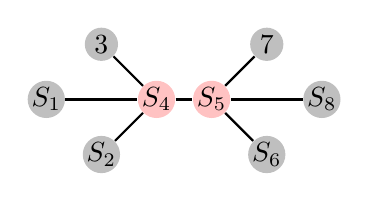
\begin{tikzpicture}[scale=0.7]
    % Draw a 7,11 network
    % First we draw the vertices
    \foreach \pos/\name in {{(1,2)/S_1}, {(2,1)/S_2}, {(2,3)/3}, {(5,1)/S_6}, {(5,3)/7}, {(6,2)/S_8}}
        \node[vertex] (\name) at \pos {$\name$};
    
    \foreach \pos/\name in {{(3,2)/S_4}, {(4,2)/S_5}}
    \node[selected vertex] (\name) at \pos {$\name$};
    
    % Connect vertices with edges 
    \foreach \source/ \dest in {S_1/S_4, S_2/S_4,3/S_4,S_4/S_5, S_5/S_6, S_5/7, S_5/S_8}
        \path[edge] (\source) -- (\dest) ;
        
\end{tikzpicture}
\end{center}



\end{itemize}

\begin{enumerate}
\item S-type 4 and S-type 5 will deviate from truthfully announce(\textbf{Free Rider Problem}). 
\item Why? They will report more S-types to save costs.
\end{enumerate}


\end{frame}




\begin{frame}
\frametitle{Result 2: APEX for $k<n$}
\begin{theorem}[$k< n$]
\label{thm_main_result}
In any \alert{acyclic} network, if $\pi$ has \alert{full support on strong connectedness}, then for repeated $k<n$ Threshold game, a {weak} APEX equilibrium {exists} whenever $\delta$ is sufficiently high.
\end{theorem}
Sketch of proof for Result 2:
\begin{enumerate}
\item The Free Rider Problem can be solved in acyclic networks.
\item An Apex equilibrium path can be constructed.
\item APEX outcome gives maximum ex-post continuation pay-off after some $T$.
\item Detectable deviation $\Rightarrow$ playing \textbf{np} forever (by off-path belief).
\item Undetectable deviation $\Rightarrow$ facing a possibility of coordination failure.
\item Any deviation will let APEX fail with positive probability.
\item Sufficiently high $\delta$ will impede deviation.
\end{enumerate}



\end{frame}


\section{Discussion}
\subsection{Discussion}





\begin{frame}
\frametitle{Extension}
\framesubtitle{Pay-off as a signal}
\begin{enumerate}

\item payoff is perfectly observed
\begin{itemize}
\item Play \textbf{p} in the first period, then the relevant information revealed.

\end{itemize}
\item payoff is noisy
\begin{itemize}
\item With full support assumption, the existing equilibrium is APEX.
\item Ex: 
\begin{itemize}
\item $u_{s_i}(a, \alert{y})$ is dependent on a random variable $\alert{y}\in \{y_1,y_2\}$
\item full support:
\begin{eqnarray*}
p_{1,\geq k} &=& \mathrm {Pr}(y=y_1|\#\textbf{p}\geq k)>0 \\
p_{1,<k} &=& \mathrm {Pr}(y=y_1|\#\textbf{p}< k)>0 \\
p_{2,\geq k} &=& \mathrm {Pr}(y=y_2|\#\textbf{p}\geq k)>0 \\
p_{2,<k} &=& \mathrm {Pr}(y=y_2|\#\textbf{p}< k)>0 
\end{eqnarray*}
\item S-type: \underline{the expected payoff on $\#\textbf{p}\geq k$} strictly larger than \underline{the expected payoff on $\#\textbf{p}< k$}
\end{itemize}




\end{itemize}


\end{enumerate}


\end{frame}


\section{Future Works}
\subsection{Future Works}


\begin{frame}

\frametitle{Further works}


\begin{enumerate}
\item Cyclic networks.
\item A general model in which players can communicate only by their actions to learn the relevant information in finite time when $\delta<1$, while the communication protocol itself is an equilibrium.
\item Equilibrium selection.  

\end{enumerate}
\end{frame}





\end{document}
